\section{环境要求}

\subsection{实验环境}
本实验的所使用的操作系统为Fedora 42 64位,Python版本为Python 3.13.5。
\begin{itemize}
    \item python:python 3.13.5
    \item 必要的python模块:
        \begin{itemize}
            \item pyecharts
            \item openpyxl
            \item pandas
        \end{itemize}
\end{itemize}

其中必要的模块都写在源代码目录下的requirenment.txt文件中。使用一下命令安装:

\begin{lstlisting}[language=fish]
pip install -r requirenment.txt
\end{lstlisting}

\begin{figure}[H]
        \centering
        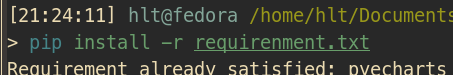
\includegraphics[width=0.7\textwidth]{./asserts/install_packages.png}
        \caption{python必要模块的安装}
\end{figure}

\section{数据源}

\subsection{数据来源}
本实验所采用的数据来源于“国家地震科学数据中心”。
